\documentclass[12pt,english]{article}
\usepackage[a4paper,bindingoffset=0.2in,%
            left=1in,right=1in,top=1in,bottom=1in,%
                        footskip=.25in]{geometry}

\usepackage{graphicx} % Required to insert images
\usepackage{amsmath}

\newcommand{\hmwkTitle}{Kalman Assignment} % Assignment title
\newcommand{\hmwkClass}{MATH-541B} % Course/class
\newcommand{\hmwkClassTime}{} % Class/lecture time
\newcommand{\hmwkAuthorName}{Saket Choudhary} % Your name
\newcommand{\hmwkAuthorID}{2170058637} % Teacher/lecturer
%----------------------------------------------------------------------------------------
%       TITLE PAGE
%----------------------------------------------------------------------------------------

\title{
\vspace{2in}
\textmd{\textbf{\hmwkClass:\ \hmwkTitle}}\\
}

\author{\textbf{\hmwkAuthorName} \\
        \textbf{\hmwkAuthorID}
        }
\date{} % Insert date here if you want it to appear below your name

\begin{document}

\maketitle
\newpage

\section{Part d}

\begin{figure}
    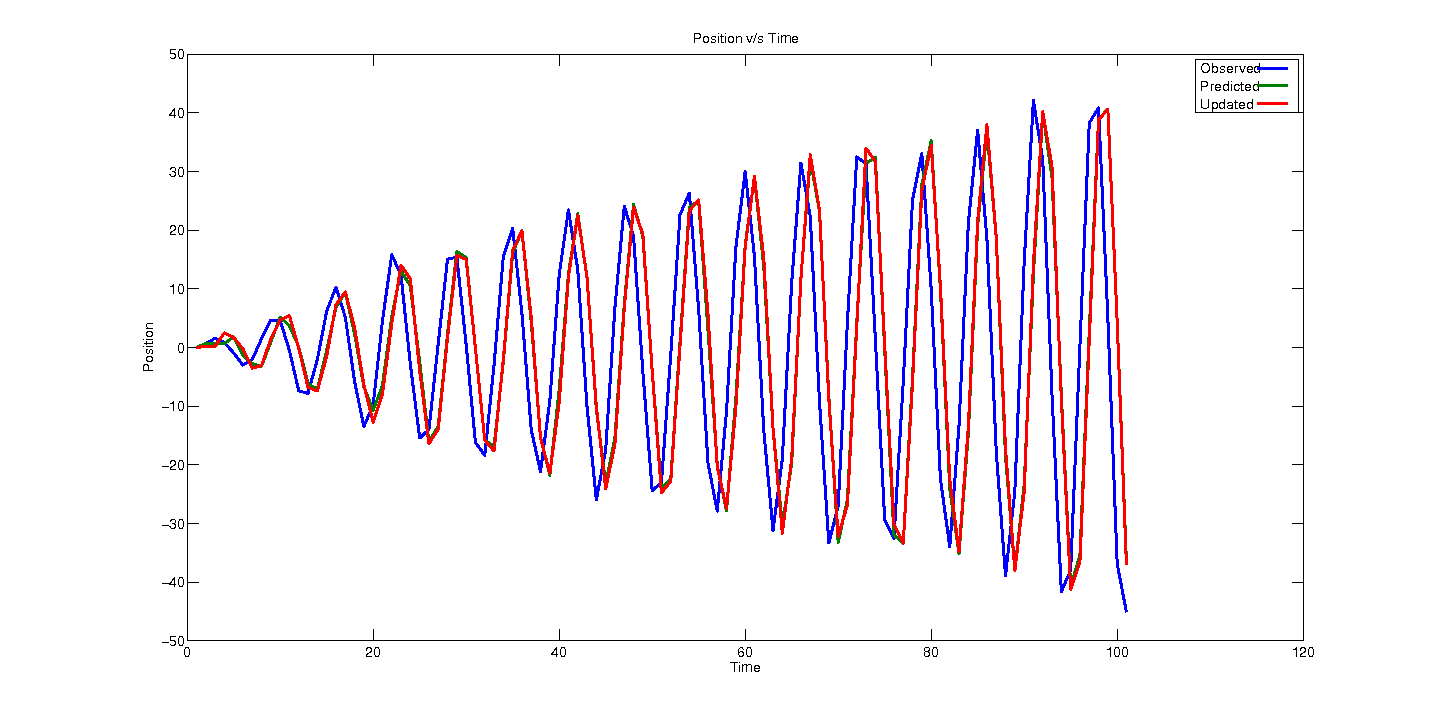
\includegraphics[width=\linewidth]{kalman-position-damping}
    \caption{Measured, predicted, filtered position with damping and resonance}
\end{figure}

\begin{figure}
    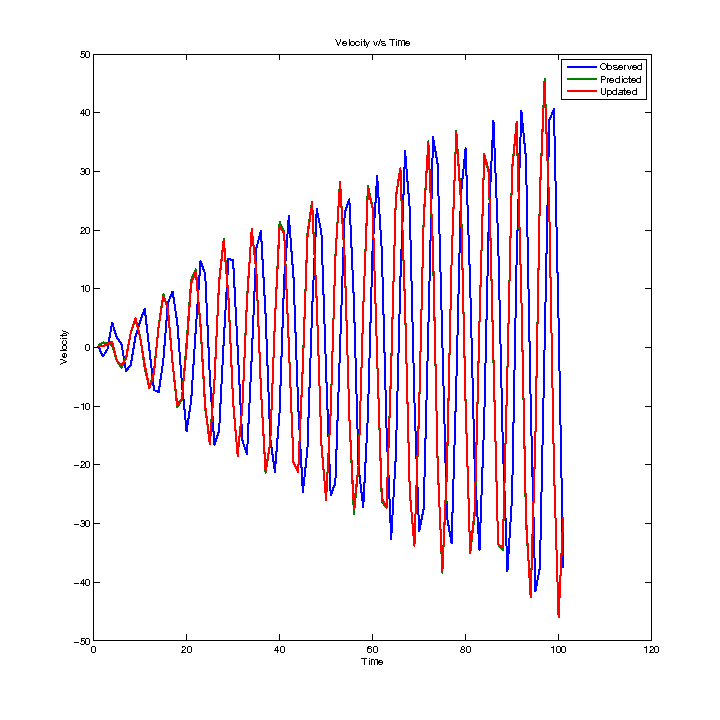
\includegraphics[width=\linewidth]{kalman-velocity-damping}
    \caption{Measured, predicted, filtered velocity with damping and resonance}
\end{figure}

\begin{figure}
    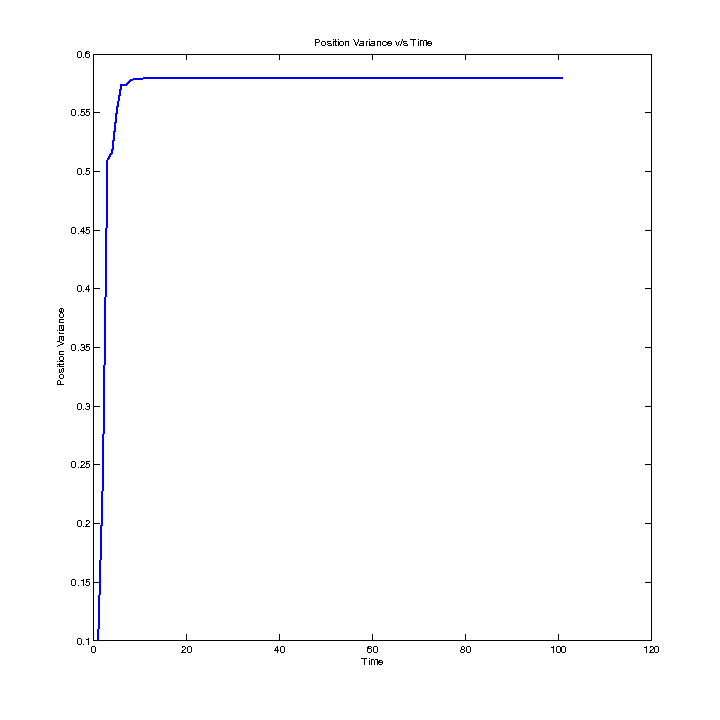
\includegraphics[width=\linewidth]{kalman-variance1-damping}
    \caption{Position variance with damping and resonance}
\end{figure}

\begin{figure}
    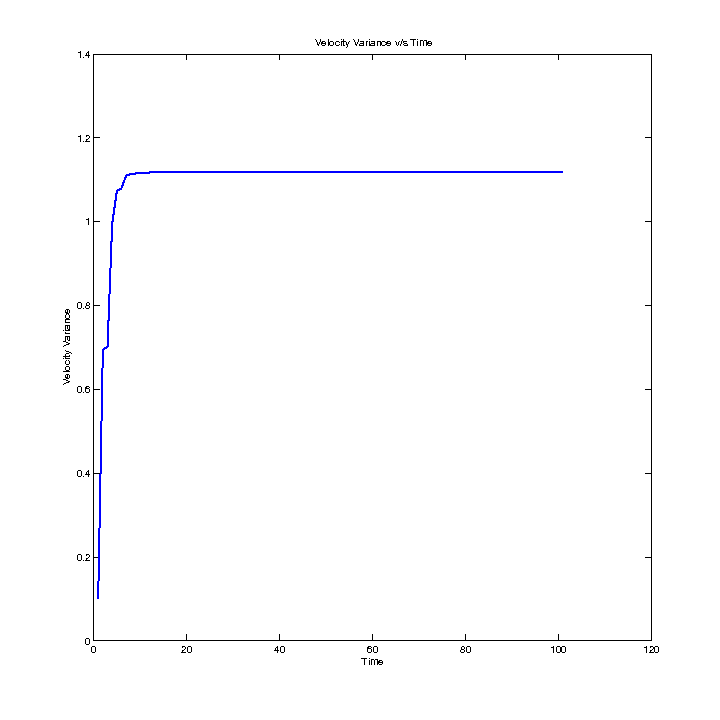
\includegraphics[width=\linewidth]{kalman-variance2-damping}
    \caption{Velocity variance with damping and resonance}
\end{figure}


For $m=100,c=1,k=1,b=1, Var(\omega)=0.1, Var(\epsilon)=0.1$


\begin{figure}
    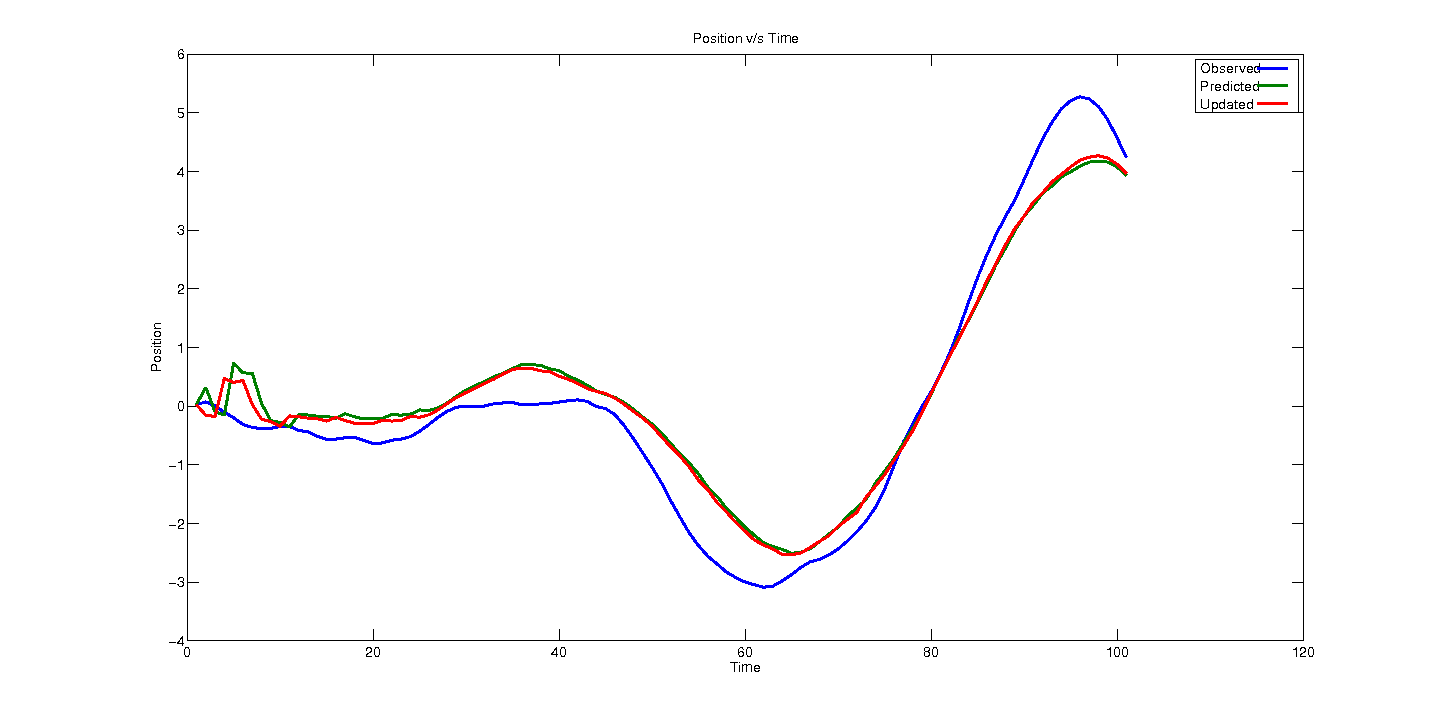
\includegraphics[width=\linewidth]{kalman-position-m100}
    \caption{Measured, predicted, filtered position with high mass}
\end{figure}

\begin{figure}
    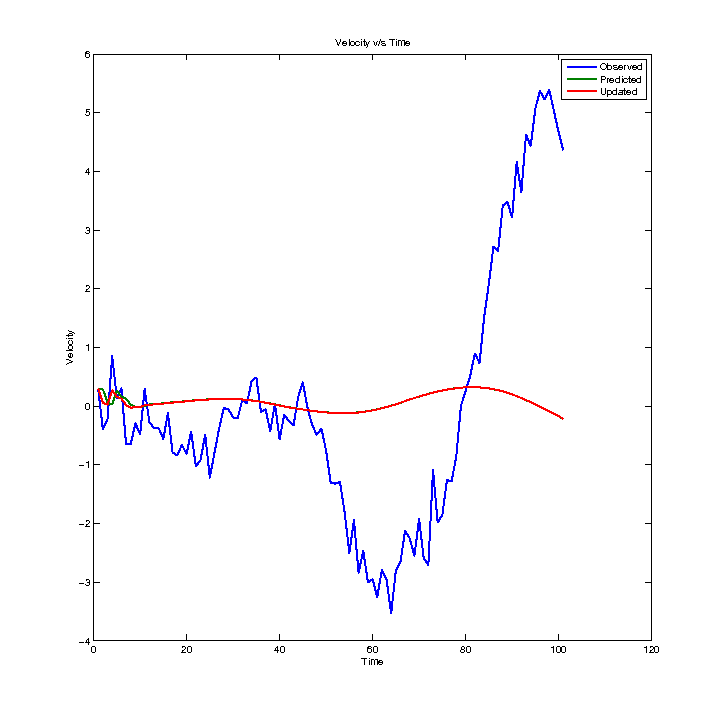
\includegraphics[width=\linewidth]{kalman-velocity-m100}
    \caption{Measured, predicted, filtered velocity with high mass}
\end{figure}

\begin{figure}
    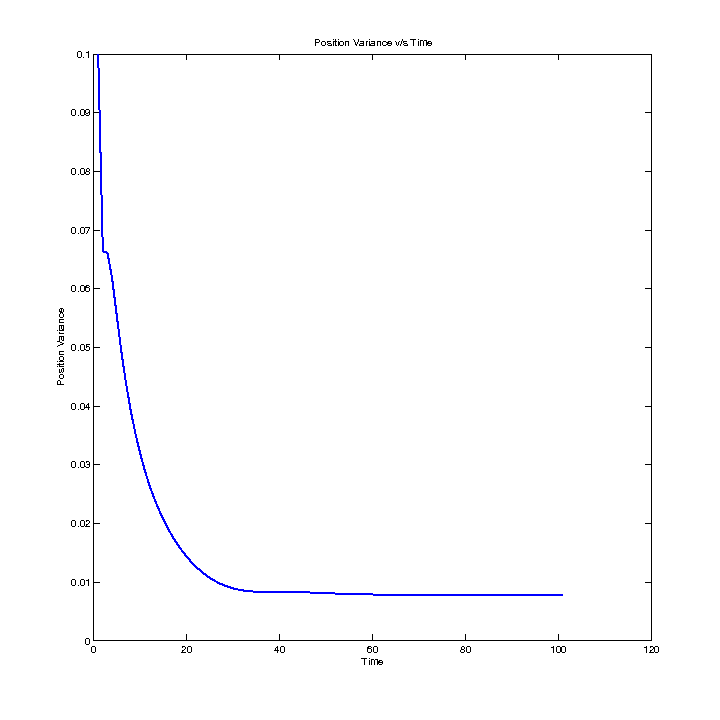
\includegraphics[width=\linewidth]{kalman-variance1-m100}
    \caption{Position variance with high mass}
\end{figure}

\begin{figure}
    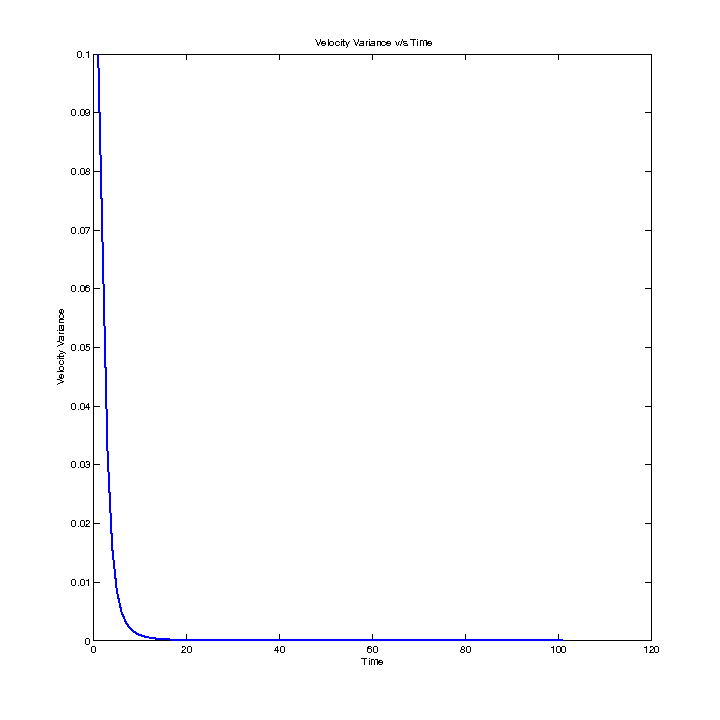
\includegraphics[width=\linewidth]{kalman-variance2-m100}
    \caption{Velocity variance with high mass}
\end{figure}


For $m=1,c=1,k=1,b=1, Var(\omega)=0.1, Var(\epsilon)=0.1$


\begin{figure}
    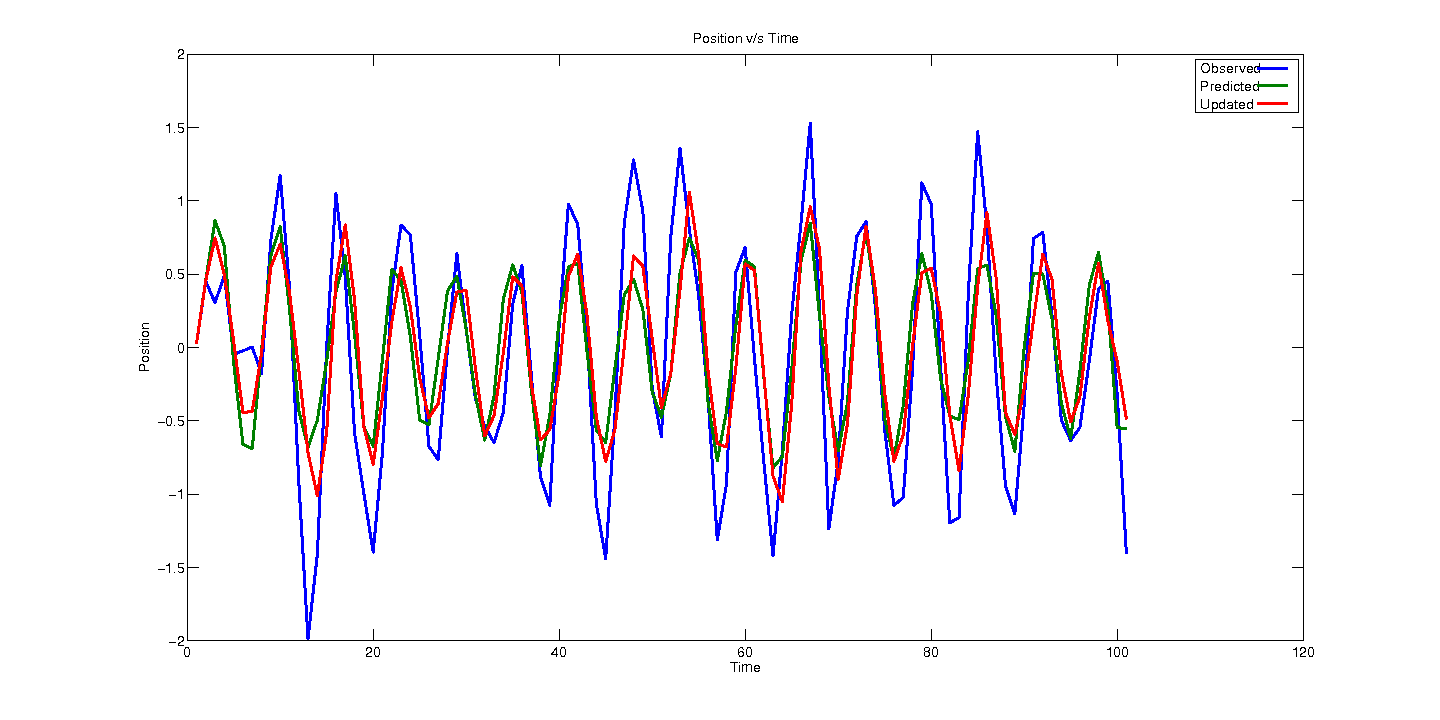
\includegraphics[width=\linewidth]{kalman-position-m1}
    \caption{Measured, predicted, filtered position with low mass}
\end{figure}

\begin{figure}
    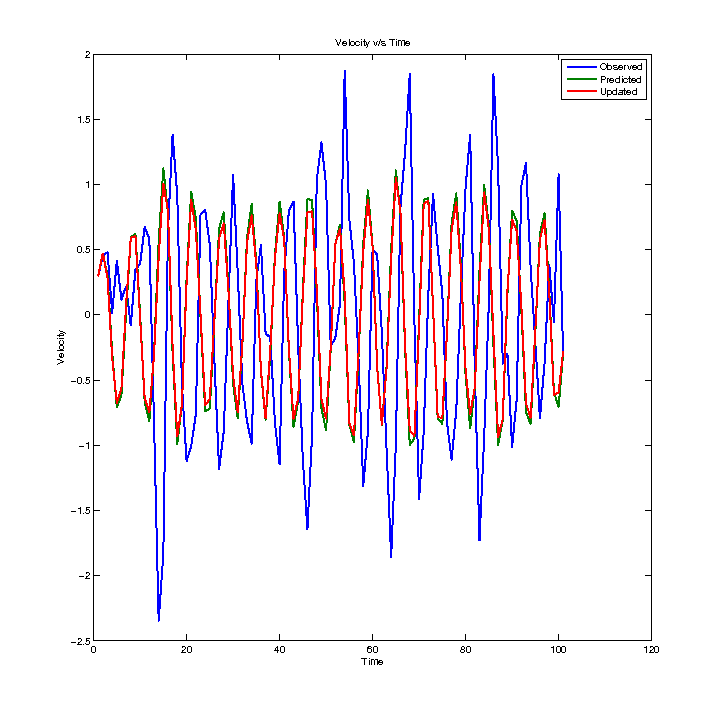
\includegraphics[width=\linewidth]{kalman-velocity-m1}
    \caption{Measured, predicted, filtered velocity with low mass}
\end{figure}

\begin{figure}
    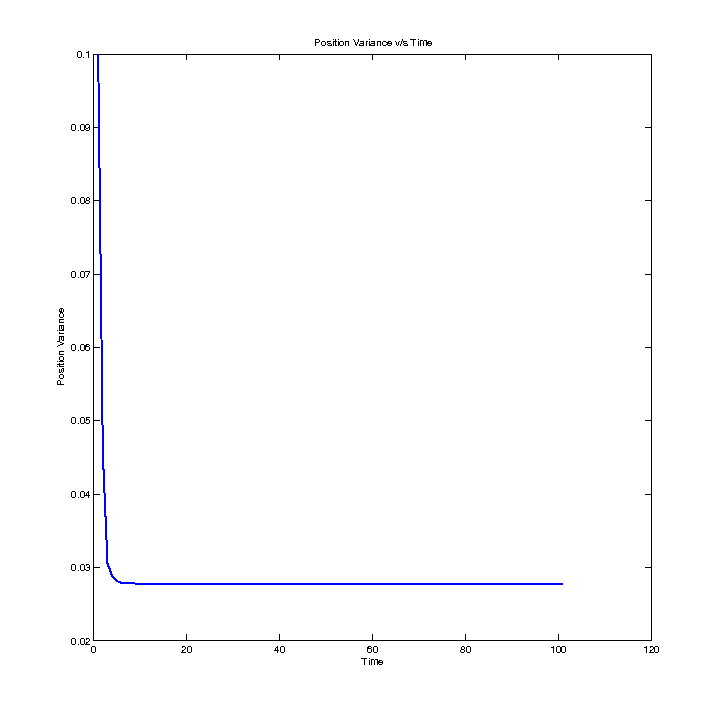
\includegraphics[width=\linewidth]{kalman-variance1-m1}
    \caption{Position variance with low mass}
\end{figure}

\begin{figure}
    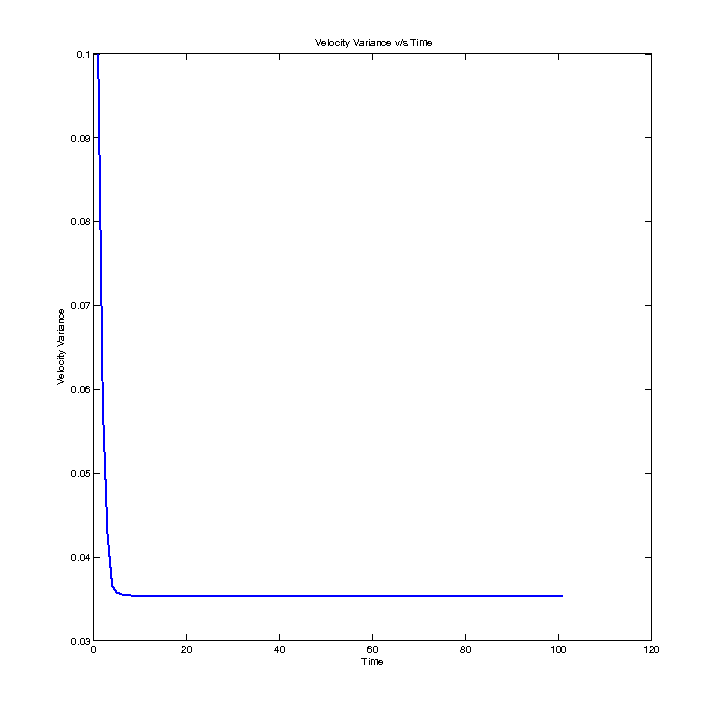
\includegraphics[width=\linewidth]{kalman-variance2-m1}
    \caption{Velocity variance with low mass}
\end{figure}


For $m=1,c=1,k=1,b=1, Var(\omega)=2, Var(\epsilon)=2$


\begin{figure}
    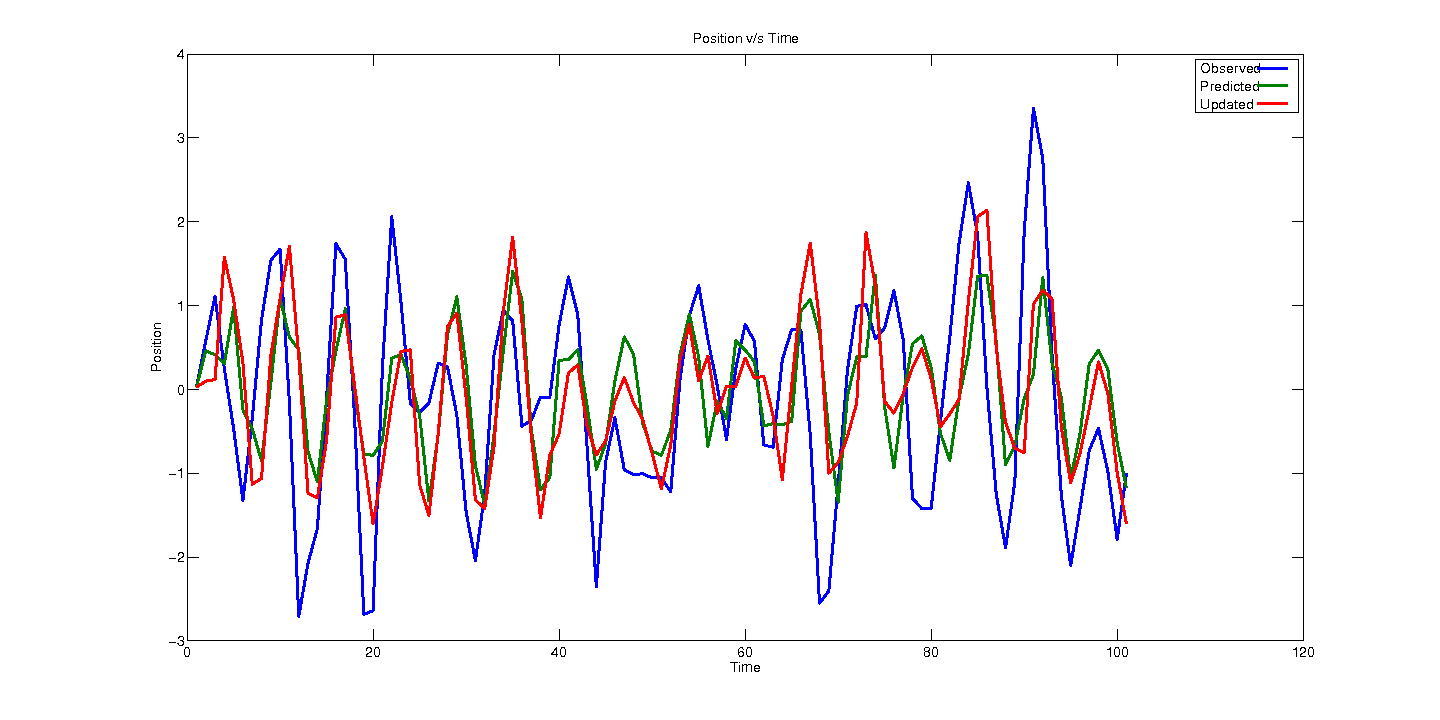
\includegraphics[width=\linewidth]{kalman-position-m1h}
    \caption{Measured, predicted, filtered position with low mass high variance}
\end{figure}

\begin{figure}
    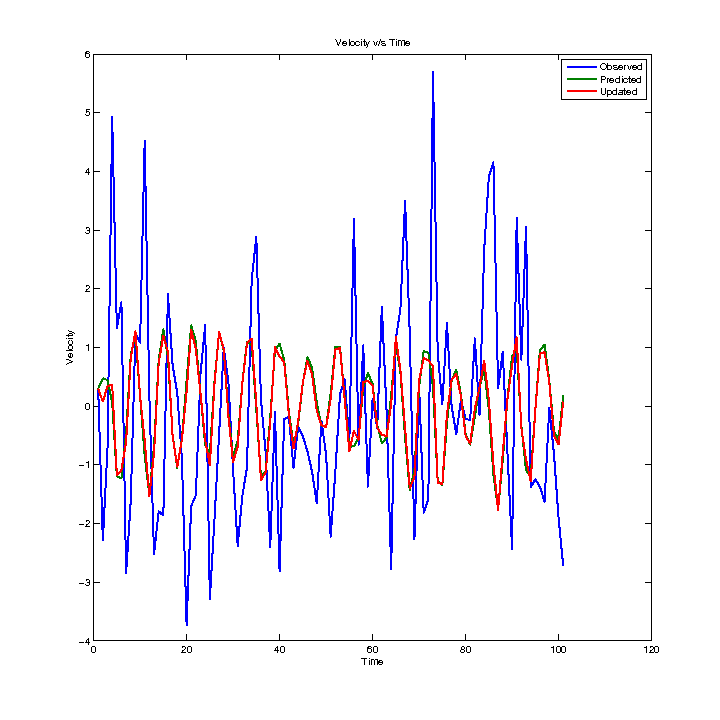
\includegraphics[width=\linewidth]{kalman-velocity-m1h}
    \caption{Measured, predicted, filtered velocity with low mass high variance}
\end{figure}

\begin{figure}
    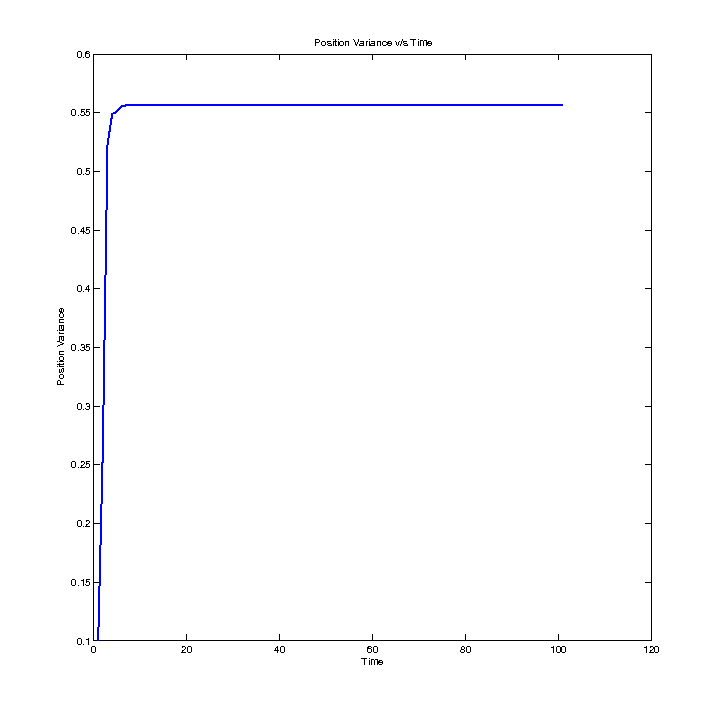
\includegraphics[width=\linewidth]{kalman-variance1-m1h}
    \caption{Position variance with low mass high variance}
\end{figure}

\begin{figure}
    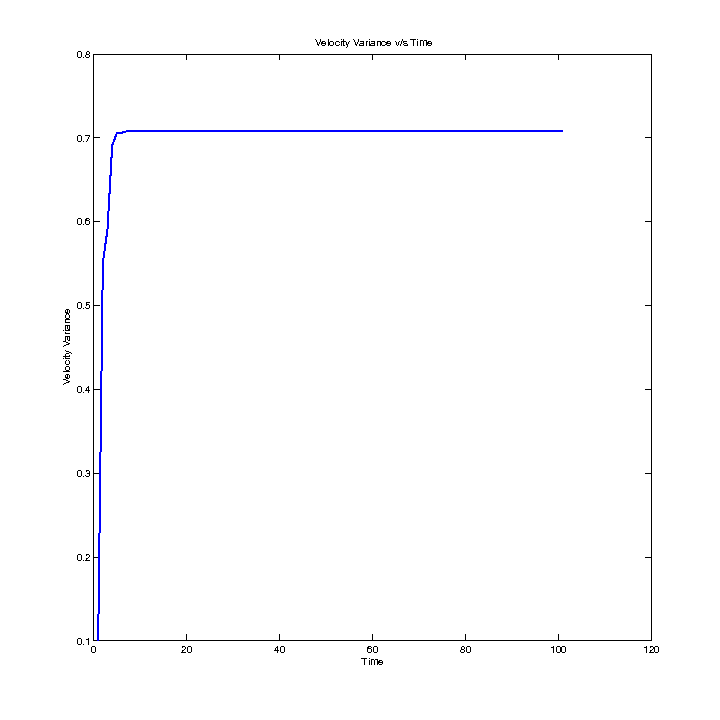
\includegraphics[width=\linewidth]{kalman-variance2-m1h}
    \caption{Velocity variance with low mass high variacne}
\end{figure}


\end{document}
